\documentclass[blue,uncompressed]{beamer}
\usepackage{tikz}
\usepackage{graphicx}
%\usepackage{listingsutf8}
\usepackage{listings}
\usepackage[spanish]{babel}
\usepackage[utf8]{inputenc}
\usepackage{multirow}
\pdfinfo
{
  /Title       (SchoolApp: Comunicación desde las aulas.)
  /Creator     (Gonzalo J. García Martín)
  /Author      (Gonzalo J. García Martín)
  /Subject     (Trabajo de Fin de Grado)
}
%%%%%%%%%%%%%%%%%%%%%%%%%%%%%%%%%%%%%%%%%%%%%%%%%%%%%%%%%%%%%%%%%%%%%%%%%%%%%%%%%%%%%%%%%%%%
% Definiendo colores para los listados de código fuente - Univ. Deusto
\definecolor{violet}{rgb}{0.5,0,0.5}
\definecolor{navy}{rgb}{0,0,0.5}
\definecolor{hellgelb}{rgb}{1,1,0.8}
\definecolor{colKeys}{rgb}{0,0,53}           %%% Todo : check color for keys
\definecolor{colIdentifier}{rgb}{0,0,0}
\definecolor{colComments}{rgb}{1,0,0}
\definecolor{colString}{rgb}{0,0.5,0}
\definecolor{lightlightgray}{rgb}{204,204,204}

\definecolor{marron}       {rgb}{0.496, 0.203, 0.152}
\definecolor{verde-claro}  {rgb}{0.625, 0.734, 0.199}
\definecolor{oscuro}       {rgb}{0.187, 0.141, 0.285}
\definecolor{gris}     	   {rgb}{0.500, 0.500, 0.500}
\definecolor{bgd-listings} {rgb}{0.999, 0.999, 0.900}
\definecolor{gray97}{gray}{.97}
\definecolor{gray75}{gray}{.75}
\definecolor{gray45}{gray}{.45}
\definecolor{gray}{gray}{.45}
%%%%%%%%%%%%%%%%%%%%%%%%%%%%%%%%%%%%%%%%%%%%%%%%%%%%%%%%%%%%%%%%%%%%%%%%%%%%%%%%%%%%%%%%%%%%
\lstloadlanguages{Java}
\lstloadlanguages{XML}
\lstset{
	float=hbp,
		language = Java,
			morekeywords={hicuda,global,alloc,shape,kernel,thread,loop_partition,tblock,over_tblock,over_thread,kernel_end,copyout,free,data,region,task,input,inout,output,pragma,omp,parallel,reduction,private,shared,target,device,copy_in,copy_out,acc,kernels,loop,copyin,copy,pcopy,pcopyin,collapse,gang,worker,independent,firstprivate,endfor,in},
				%\emph      ={omp,parallel,reduction,private,shared},
				xleftmargin=5.0ex,    % Margen izq. para que los números de línea se vean
				emphstyle=\textbf,
        basicstyle=\ttfamily\scriptsize,
        identifierstyle=\color{colIdentifier},
        keywordstyle=\color{colKeys},
        stringstyle=\color{colString},
        commentstyle=\color[rgb]{0.133,0.545,0.133},
        columns=flexible,
        tabsize=4,
        frame=single,
        extendedchars=true,
        showspaces=false,
        showstringspaces=false,
        numbers=left,
        numberstyle=\tiny,
        breaklines=true,
        backgroundcolor=\color{lightlightgray},
        breakautoindent=true,
        captionpos=b
        morecomment=[l][\color{colKeys}]{\#}
}
%%%%%%%%%%%%%%%%%%%%%%%%%%%%%%%%%%%%%%%%%%%%%%%%%%%%%%%%%%%%%%%%%%%%%%%%%%%%%%%%%%%%%%%%%%%%
\mode<handout>
{
	\usepackage{pgfpages}
	\pgfpagesuselayout{2 on 1}[a4paper,border shrink=5mm]
	\setbeamercolor{background canvas}{bg=black!0}
	\setbeameroption{show notes}
}

\mode<presentation>
{
	\usetheme{Madrid}
	\usecolortheme{ull}
	\setbeamercovered{transparent}
	%\logo{  % Logo ULL en esquina inferior derecha
	%    \includegraphics[width=.25\textwidth]{FIGURES/logoull-oficial.png}
	%}
}
%%%%%%%%%%%%%%%%%%%%%%%%%%%%%%%%%%%%%%%%%%%%%%%%%%%%%%%%%%%%%%%%%%%%%%%%%%%%%%%%%%%%%%%%%%%%
\AtBeginSection[]
{
	\begin{frame}<beamer>
		\frametitle{Outline}
		\tableofcontents[currentsection,currentsubsection]
	\end{frame}
}
%%%%%%%%%%%%%%%%%%%%%%%%%%%%%%%%%%%%%%%%%%%%%%%%%%%%%%%%%%%%%%%%%%%%%%%%%%%%%%%%%%%%%%%%%%%%
\title{\textbf{SchoolApp}}
\subtitle{Comunicación desde las aulas}
\author[Gonzalo J. García Martín]
{
	\textbf{Gonzalo J. García Martín}
	%\alert{Francisco~de Sande} \\
	%\url{fsande@ull.es}
}
\institute[ULL]

\date[Trabajo de Fin de Grado]{\textsc{Trabajo de Fin de Grado}     \\
                           La Laguna, 23 de Septiembre, 2015}
\subject{TFG}

\AtBeginSection[]
{
	\frame<handout:0>
		{
			\frametitle{Índice}
			\tableofcontents[current]
		}
}
%%%%%%%%%%%%%%%%%%%%%%%%%%%%%%%%%%%%%%%%%%%%%%%%%%%%%%%%%%%%%%%%%%%%%%%%%%%%%%%%%%%%%%%%%%%%
\newcommand{\SchollApp}{\texttt{SchoolApp{}}}

\setbeamerfont{title}{size=\Large,shape=\sffamily}
\setbeamerfont{author}{size=\small,shape=\sffamily}
\setbeamerfont{institute}{size=\scriptsize,shape=\sffamily}
\setbeamerfont{date}{size=\scriptsize,shape=\sffamily}
%%%%%%%%%%%%%%%%%%%%%%%% Title Page %%%%%%%%%%%%%%%%%%%%%%%%%%%%%%%%%%%%%%%%%%%%%%%%%%%%%%%%%%%%%%%%%%%%
\defbeamertemplate*{title page}{AGH}[1][]
{
  \vbox{}
  %\vspace*{2.3cm}
  \vfill 
\includegraphics[width=0.15\linewidth]{Images/logos/logo_vertical}
    \vfill
  %\hspace*{1.8cm}
  \begin{columns}
    \begin{column}{0.6\textwidth}
      \begin{beamercolorbox}[sep=8pt,#1]{title}
	\centering{\usebeamerfont{title}\inserttitle\par}
	\ifx\insertsubtitle\@empty%
	\else%
	  \vskip0.25em%
	  {\usebeamerfont{subtitle}\usebeamercolor[fg]{subtitle}\insertsubtitle\par}%
	\fi%
	
      \end{beamercolorbox}%
      \vskip1em\par
      \hspace*{2.35cm}
      \begin{beamercolorbox}[sep=8pt,#1]{author}
	\usebeamerfont{author}\insertauthor
      \end{beamercolorbox}
      \vskip1em\par
      \hspace*{2.35cm}
      \begin{beamercolorbox}[sep=8pt,#1]{institute}
	\usebeamerfont{institute}\insertinstitute
      \end{beamercolorbox}
      \hspace*{2.35cm}
      \begin{beamercolorbox}[sep=8pt,#1]{date}
	\usebeamerfont{date}\insertdate
      \end{beamercolorbox}\vskip0.5em
    \end{column}
    
    \begin{column}{0.4\textwidth}
      \hfill 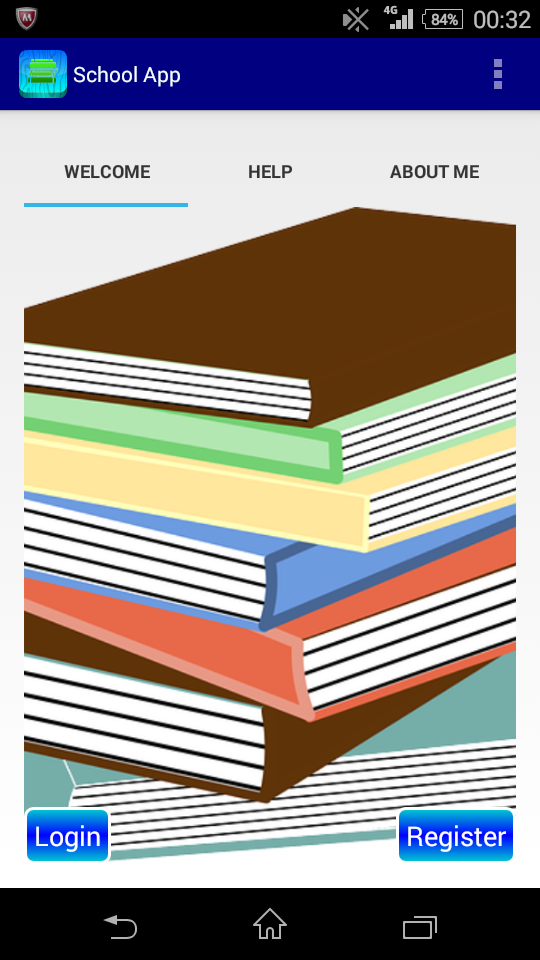
\includegraphics[width=0.8\linewidth]{Images/App/welcome.png}
    \end{column}
  \end{columns}
    %\hfill \includegraphics[width=0.2\linewidth]{Images/varios/MainActivity.png}
    %{\usebeamercolor[fg]{titlegraphic}\inserttitlegraphic\par}
	%	\vfill \includegraphics[width=0.3\linewidth]{FIGURES/logos/nwo}
	%	\hfill \includegraphics[width=0.17\linewidth]{FIGURES/logos/stw}
	%	\hfill \includegraphics[width=0.2\linewidth]{FIGURES/logos/ipn.jpg}
  %\vfill
}
%%%%%%%%%%%%%%%%%%%%%%%%%%%%%%%%%%%%%%%%%%%%%%%%%%%%%%%%%%%%%%%%%%%%%%%%%%%%%%%%%%%%%%%%%%%%
% Slide numbers. 
%\expandafter\def\expandafter\insertshorttitle\expandafter{%
%  \insertshorttitle\hfill%
%  \insertframenumber\,/\,\inserttotalframenumber
%}
%%%%%%%%%%%%%%%%%%%%%%%%%%%%%%%%%%%%%%%%%%%%%%%%%%%%%%%%%%%%%%%%%%%%%%%%%%%%%%%%%%%%%%%%%%%%
\begin{document}
	%\frame{\titlepage}
	\begin{frame}[plain]
	\titlepage
	\end{frame}

	\frame{\frametitle{Índice}\tableofcontents}
		\section{Introducción}
			\begin{frame}
    \frametitle{Introducción}
    %\block{Objetivo del TFG}
    \begin{itemize}
	\item \textbf{Tutor académico:} Francisco de Sande González
        \item \textbf{Línea de trabajo del proyecto:} Programación de aplicaciones interactivas en {\it Android}.
    \end{itemize}
    %\endblock{}
        {\usebeamercolor[fg]{titlegraphic}\inserttitlegraphic\par}
		\vfill 
\includegraphics[width=0.2\linewidth]{Images/logos/remind_logo_2}
		\hfill %
		
\includegraphics[width=0.2\linewidth]{Images/logos/miColegioApp}
		\hfill 
\includegraphics[width=0.35\linewidth]{Images/logos/android_logo}
\end{frame}
% -------------------------------------------------------------------------
\begin{frame}
	\frametitle{Introducción}
	\block{Objetivos}
		\begin{itemize}
			\item Conocimientos del Grado en Ingeniería Informática.
			\item Conocimientos sobre {\it Android}.
			\item Diseño y desarrollo de un proyecto.
			\item Conocimientos sobre el uso de servicios en la nube y su utilización en aplicaciones {\it Android}.
			\item Repositorio online.
			\item Creación de una memoria técnica.
			\item \LaTeX{}.
		\end{itemize}
	\endblock{}
\end{frame}
% -------------------------------------------------------------------------
		\section{Especificación de Requisitos}
			\begin{frame}
	\frametitle{Especificación de Requisitos}
	\begin{columns}
		\begin{column}{0.6\textwidth}
			\block {Funcionalidades}
			\begin{itemize}
				\item Registro (Roles).
				%\item Acceso.
				%\item Recuerdo de la contraseña.
				\item Contactos.
				%\item Chat.
				\item Notificaciones.
				\item Circulares.
				%\item Citas.
				%\item Visualización de datos.
				\item Modificación de datos.
				\item Baja de Usuario.
			\end{itemize}
			\endblock{}
		\end{column}
		\begin{column}{0.4\textwidth}
			\vfill 
			\begin{center}
				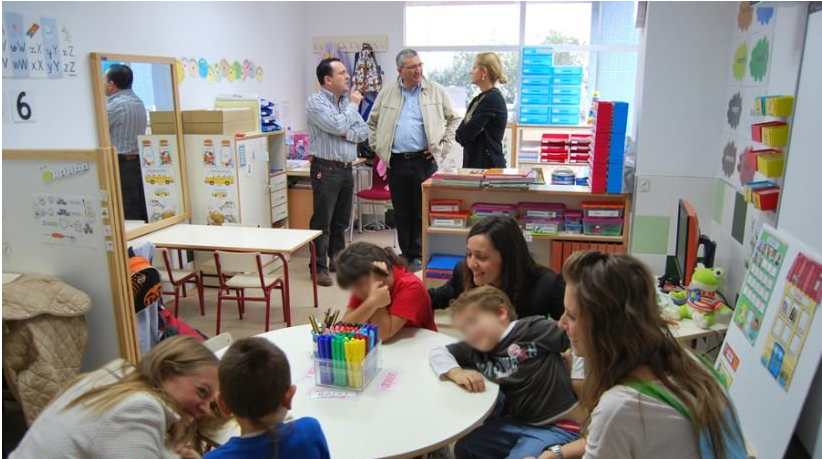
\includegraphics[width=0.9\linewidth]{Images/padresProfesNinos}
			\end{center}
		\end{column}
	\end{columns}
\end{frame}

%--------------------------------------------------------------------

\begin{frame}
	\frametitle{Especificación de Requisitos}
	\block {Comunicaciones Permitidas}
		\begin{table} [!hbt]
			\begin{center}
				\begin{tabular}{|| c | c | c | c ||}
					\hline
					\hline
					& Padre & Alumno & Profesor \\
					\hline
					Padre & Mensajes & - & Mensajes \\
					\hline
					Alumno & - & Mensajes & Mensajes \\
					\hline
					Profesor & Circulares y Mensajes & Circulares y Mensajes & Mensajes \\
					\hline
					\hline
				\end{tabular}
			\end{center}
		\end{table}
	\endblock{}
\end{frame}
		\section{Herramientas Software}
			\begin{frame}
	\frametitle{Herramientas de Software}
	\block{{\it Android Studio}: \texttt{http://developer.android.com/sdk}}
		\begin{itemize}
			\item Entorno de desarrollo integrado.
			\item Uso intuitivo.
			\item Ligero.
		\end{itemize}
	\endblock{}
	\block{\it Tutoriales}
		\begin{itemize}
			\item {\it Suporting different devices}.
			\item {\it Building a dynamic UI with fragments}.
			\item {\it ActionBar Tab Swipe}.
			\item {\it TabHost Swipe}.
			\item {\it Adding animations}.
			\item {\it Expandable ListView}.
		\end{itemize}
	\endblock{}
\end{frame}

%------------------------------------------------------------------

\begin{frame}
	\frametitle{Herramienta Software}
	\block{\it Firebase}
		\begin{itemize}
			\item Proveedor de contenidos.
			\item Ofrece servicios en la nube.
			\item Seguro y sencillo (Funcionalidades).
			\item Datos tipo JSON.
			\item Consturucción de datos en tiempo real.
			\item Interfaz de programación de aplicaciones de seguridad basada en la expresión altamente flexible.
		\end{itemize}
	\endblock{}
	\block{\it Tutorial}
		\begin{itemize}
			\item {\it Firebase Storage}: \\ {\texttt{https://www.firebase.com/docs/android/guide/}}
		\end{itemize}
	\endblock{}
\end{frame}

%------------------------------------------------------------------

\begin{frame}
	\frametitle{Herramientas de Software}
	\block{\it Parse}
		\begin{itemize}
			\item Proveedor de servicios en la nube.
			\item Alternativa a {\it Firebase}.
			\item Utiliza datos SQL.
			\item Múltiples SDK.
			\item Notificaciones tipo {\it Push}.
		\end{itemize}
	\endblock{}
	\block{\it Tutorial}
		\begin{itemize}
			\item {\it Parse Storage}:\\ {\texttt{http://www.sitepoint.com/creating-cloud-backend-android\\-app-using-parse/}}
		\end{itemize}
	\endblock{}
\end{frame}
		\section{Descripción de \SchollApp}
			\begin{frame}
	\frametitle{Aplicaciones Similares}
	\begin{columns}
		\begin{column}{0.6\textwidth}
			\block{\it Remind}
				\begin{itemize}
					\item Forma sencilla de enviar mensajes a estudiantes y padres.
					\item Los profesores, monitores o administradores pueden enviar recordatorios, deberes o mensajes motivadores.
					\item Seguro, teléfonos confidenciales.
					\item Los profesores pueden enviar anuncios o mensajes tipo chat.
				\end{itemize}
			\endblock{}
		\end{column}
		\begin{column}{0.4\textwidth}
			\hfill 
\includegraphics[width=0.7\linewidth]{Images/Remind.png}
		\end{column}
	\end{columns}
\end{frame}

%------------------------------------------------------------------

\begin{frame}
	\frametitle{Aplicaciones Similares}
	\begin{columns}
		\begin{column}{0.6\textwidth}
			\block{\it miColegioApp}
			\begin{itemize}
				\item El colegio contrata los servicios.
				\item Registro de usuarios.
				\item Introducir el código del centro en la aplicación.
				\item Se asocian a los usuarios con un centro.
				\item Los usuarios pueden recibir notificaciones, circulares y boletines.
			\end{itemize}
			\endblock{}
		\end{column}
		\begin{column}{0.4\textwidth}
			\hfill 
\includegraphics[width=0.7\linewidth]{Images/miColegioApp.png}
		\end{column}
	\end{columns}
\end{frame}

%------------------------------------------------------------------
\begin{frame}
	\frametitle{Descripción}
	\block{Definición de términos}
		\begin{itemize}
			\item {\it Activity}.
			\item {\it Fragment}.
			\item {\it Dialog}.
		\end{itemize}
	\endblock{}
	
	{\usebeamercolor[fg]{titlegraphic}\inserttitlegraphic\par}
	\vfill 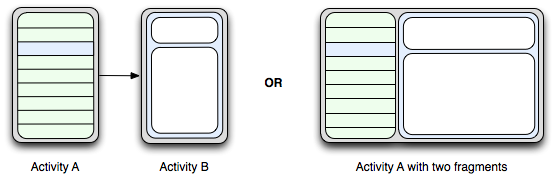
\includegraphics[width=0.7\linewidth]{Images/android_fragments}
	\hfill 
\includegraphics[width=0.25\linewidth]{Images/dialog}
	
\end{frame}

%------------------------------------------------------------------

%Estilo de este frame portrait (hoja normal posición de folio)
\begin{frame}
	\frametitle{Descripción}
	\begin{center}
		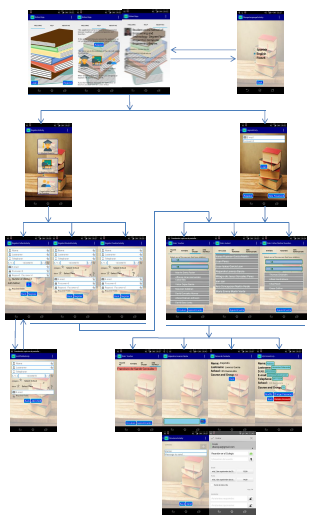
\includegraphics[width=0.3\linewidth]{Images/mapaActividades.png}
	\end{center}
\end{frame}

%------------------------------------------------------------------

\begin{frame}
	\frametitle{Descripción}
	\block{}
		Vídeo ilustrativo del funcionamiento de la aplicación.
	\endblock{}
\end{frame}
		\section{Desarrollo de la Aplicación}
			\begin{frame}
	\frametitle{Desarrollo de la Aplicación}
	\block{Clases Principales}
		\begin{itemize}
			\item Clase {\ttfamily Student}.
			\item Clase {\ttfamily Father}.
			\item Clase {\ttfamily Teacher}.
			\item Clase {\ttfamily Message}.
			\item Clase {\ttfamily MessageSQLHelper}.
		\end{itemize}
	\endblock{}
\end{frame}

%--------------------------------------------------------------------

\begin{frame}
	\frametitle{Descripción}
	\block{}
		Descripción del proyecto en {\it Android Studio}.
		{\ttfamily MessageSQLHelper} e interacción con la Base de Datos de {\it Frebase}.
	\endblock{}
\end{frame}

%--------------------------------------------------------------------
		\section{Problemas}
			\begin{frame}
	\frametitle{Problemas}
	\block{Problemas}
		\begin{enumerate}
			\item {\it Android Studio} no render Target.
			\item Fallo al encontrar {\ttfamily com.android.support:appcompat-v7:16.+}.
			\item Fallo al encontrar {\it Java}
			\item Duplicidad en la dependencias de los paquetes.
			\item Fallo al encontrar {\ttfamily com.android.support:support-v13}.
			\item Arregle {\ttfamily Gradle} (Fix {\ttfamily Gradle}).
			\item {\it SDK} no encontrado.
			\item Consultas a la espera de modificación de datos.
		\end{enumerate}
	\endblock{}
\end{frame}
		%\section{Despliegue}	
			%\begin{frame}
	\frametitle{Despliegue}
	
\end{frame}
		\section{Summary and conclusions}
			\begin{frame} [fragile]
	\frametitle{Summary and conclusions}
	\block{Conclusions}
		The realization of this project will apply the expertise gained during the years of study, allowing real assimilation of the necessary skills and acquire new knowledge.
		
		\bigskip
		This experience discloses the level of involvement that implies creating a fully functional application in a real environment.
		
		\bigskip
		The analysis of other similar applications can realize the state of the market for the type of application built.
	\endblock{}
\end{frame}
		\include{Capitulos/Cap9_final}
%%%%%%%%%%%%%%%%%%%%%%%%%%%%%%%%%%%%%%%%%%%%%%%%%%%%%%%%%%%%%%%%%%%%%%%%%%%%%%%%%%%%%%%%%%%%
\end{document}